\documentclass[10pt,twocolumn,letterpaper]{article}
\usepackage[pagenumbers]{cvpr}
\usepackage{graphicx}
\usepackage{amsmath,amssymb}
\usepackage{booktabs}
\usepackage[breaklinks,colorlinks,bookmarks=false,citecolor=blue,linkcolor=red]{hyperref}
\usepackage[capitalize]{cleveref}

\def\paperID{0000}
\def\confName{CS131}
\def\confYear{2026}

\title{What Actually Works at 10\,m? An Honest Study of Static, Texture, and Blade-Motion Cues for Wind-Turbine Detection in Sentinel-2}

\author{%
[Author One] \quad [Author Two] \quad [Author Three]\\
Stanford University, CS131\\
{\tt\small \{author1, author2, author3\}@stanford.edu}
}

\begin{document}
\maketitle

\begin{abstract}
We ask a narrow, practical question: at Sentinel-2's 10\,m ground sample distance, which computer-vision cues actually separate operating wind turbines from background, and which only appear to? We build a clean, leakage-free benchmark of 173 U.S.\ wind projects across 35 states with project-grouped train/test splits and a single locked evaluation, and we compare four cue families head to head: from-scratch CS131 static primitives (Gaussian, Sobel, Hough, Harris, matched template), a static brightness-salience score, a HOG+SVM appearance baseline, and a novel \emph{band-parallax} cue that exploits Sentinel-2's staggered inter-band acquisition to read blade motion. The parallax cue, on its own, reaches held-out per-project AUC 0.952 and is the most salience-robust family on the bright, textured terrain where appearance cues fail; fusing it with salience reaches 0.971. Controlled tests show the cue carries motion information that is separable from contrast, which no prior work has demonstrated. We are equally explicit about limits: run as a real detector rather than a candidate-point classifier, the same model scores only F1 0.39 with count $R^2$ 0.13, and the cue is blind to idle turbines. The contribution is a rigorous, interpretable accounting of what each cue is worth at 10\,m, not a new state-of-the-art detector.
\end{abstract}

\section{Introduction}
Knowing where wind turbines are, and whether they are turning, matters for grid operations, renewable-capacity tracking, and energy-market and carbon analysis. A concrete and fast-growing case is data-center investment: hyperscale and AI data centers are enormous, rapidly expanding electricity loads whose siting, valuation, and clean-power claims increasingly turn on the renewable supply around them, and an installed-capacity map cannot tell an investor how much of the nearby wind is actually generating. Pairing a free, repeatable read of which turbines are spinning with their nameplate capacity lets one estimate the operational wind share feeding a project's grid region or contracted portfolio, and independently test its renewable-power claims. More broadly, official inventories such as the USGS U.S.\ Wind Turbine Database (USWTDB)~\cite{uswtdb} and EIA Form 860 update on long lags, and the sub-meter aerial imagery that makes turbines easy to see is flown only every few years, so it cannot nowcast. Sentinel-2 is free, global, and revisits every five days, which makes it the natural sensor for a near-real-time signal, but its 10\,m resolution is the catch: a turbine spans only a few pixels, and on bright or textured ground it is spatially resolved yet not locally salient. A purely appearance-based detector therefore fails on most scenes, which is the central challenge we confront.

This paper is deliberately framed as an honest comparison rather than a leaderboard push. We treat the task as candidate-point classification (given a location, is there an operating turbine?) so that every cue is evaluated on identical inputs, and we add a real detection-mode evaluation to expose the gap between ranking and detecting. Our contributions are: (1) a clean, project-grouped, single-locked-test benchmark at 10\,m; (2) a controlled comparison of four cue families implemented from scratch; (3) a novel, interpretable band-parallax (blade-motion) cue, with controls showing it is separable from contrast; and (4) a frank account of where each method works, where it breaks, and why. We deliberately study cue \emph{effectiveness} in isolation rather than chasing a single headline number, because the most useful finding for a 10\,m practitioner is which signals are worth computing at all.

\section{Related Work}
\textbf{Mapping products.} Microsoft's Global Renewables Watch~\cite{grw} maps turbines globally from 4.7\,m PlanetScope basemaps, reaching object precision 90.8/recall 81.6/F2 83.3 and country-level count $r^2{=}0.932$; its labels derive from the OpenStreetMap-based registry of Dunnett \etal~\cite{dunnett}. Satlas~\cite{satlas} reports count $r^2{=}0.978$. These are object/count products at finer resolution, not 10\,m per-instance studies, and neither uses a motion cue.

\textbf{Sentinel-2 10\,m classical detectors.} Mandroux \etal~\cite{mandroux_ipol,mandroux_isprs} detect turbines on Sentinel-2 with an a-contrario shadow-and-hub model, reaching mAP 0.939 on a favorable scene but 40--60\% recall at country scale. Crucially, they use the blue band B02 \emph{only}, ``to avoid blurring effects due to rotating blades.'' We do the opposite: the blade blur is our signal. He \etal~\cite{he2025} map turbines across China from Sentinel-2 at 10\,m, the closest setting to ours on imagery and region, but again from static appearance.

\textbf{Band-motion methods.} Sentinel-2's detectors are offset on the focal plane, so bands are exposed at slightly different times; Heiselberg~\cite{heiselberg} first used this parallax to measure aircraft and ship velocities, and Liu \etal~\cite{liu} extended it to a hybrid aircraft detector. Nahrstedt \etal~\cite{nahrstedt} are the only prior work applying the cue to turbines, training a DenseNet that reports a single in-distribution validation accuracy near 99.4\% with a degenerate negative class and no AUC, F1, held-out test, or grouped split.

\textbf{High-resolution and offshore detectors.} YOLO-style detectors on sub-meter imagery~\cite{wtyolo} and offshore SAR detectors~\cite{deepowt} perform well but in easier regimes (sub-meter, or near-trivial water backgrounds) that are not comparable to onshore 10\,m optical.

\textbf{How we differ.} Against the static 10\,m detectors we add the motion cue they discard; against the one prior motion method we replace a black-box accuracy with an interpretable, contrast-controlled, grouped-split quantification; and against the mapping products we make no counting claim, instead measuring per-cue effectiveness and reporting our own honest object-level number.

\begin{figure}[t]
\centering
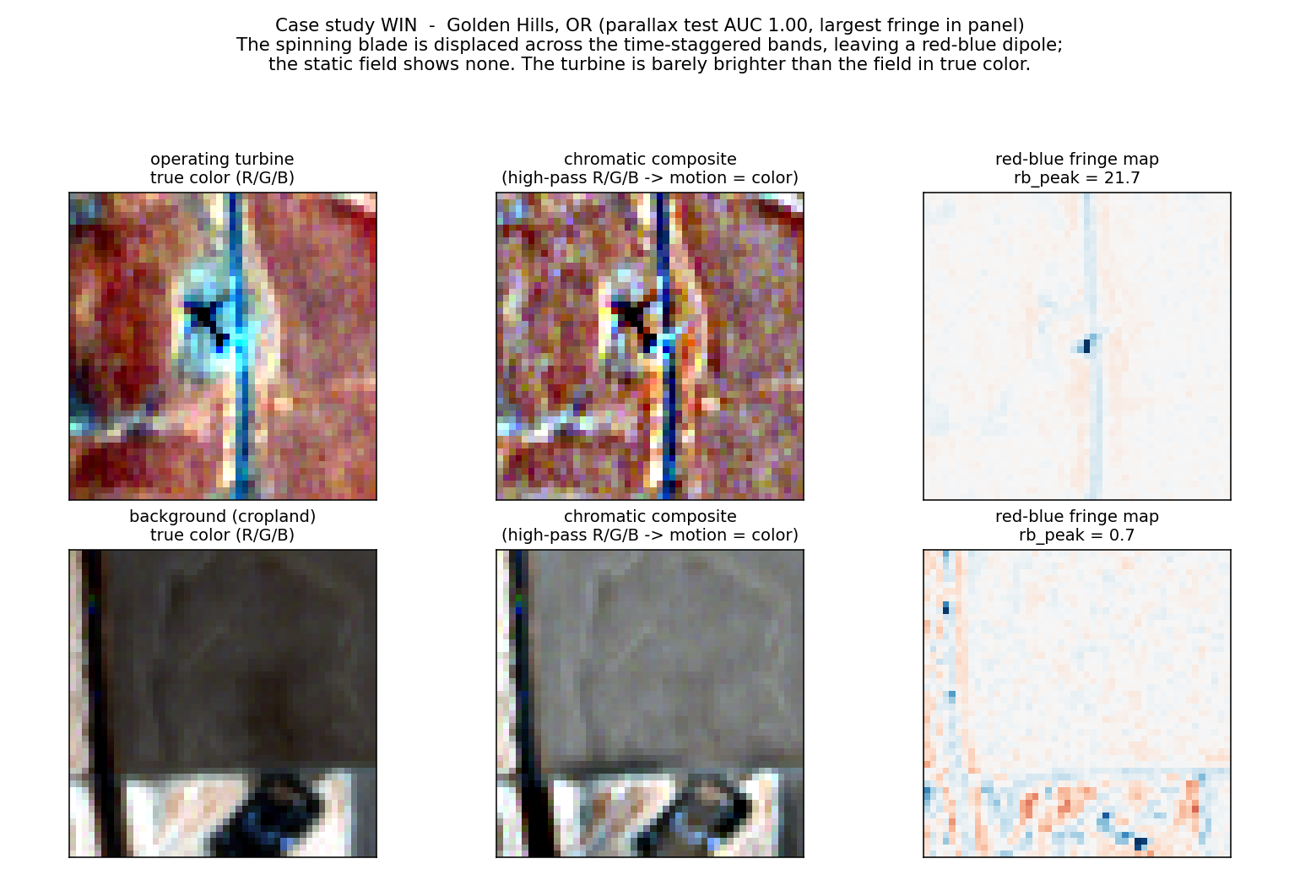
\includegraphics[width=\linewidth]{figs/fig_hero.png}
\caption{The band-parallax mechanism on real Sentinel-2 pixels (Golden Hills, OR). Top: an operating turbine is barely brighter than the field in true color, yet the spinning blade is displaced across the time-staggered bands and leaves a bright smear and a sharp red-blue dipole. Bottom: a background field shows no such fringe.}
\label{fig:hero}
\end{figure}

\section{Methodology}
\textbf{Data and split.} Ground truth is USWTDB high-confidence locations. We select 173 projects on metadata alone (35 states, commissioned 2008--2023 so all are operational in 2024 imagery), then pull the lowest-cloud summer-2024 scene per project and cut 48$\times$48 R/G/B/NIR patches at 10\,m: 5{,}339 turbine-centered positives and 5{,}295 background negatives ($\geq$500\,m from any turbine), 10{,}634 patches over 171 projects. The split is grouped by whole project (139 train / 33 test with patches), so no farm is split, and is stratified by census region and vintage. All development uses train-only GroupKFold cross-validation with standardization fit inside each fold; the test split is scored exactly once.

\textbf{Cue families.} Each patch yields four feature families. (i) \emph{CS131 static primitives} (4 features): center Sobel gradient energy, max Harris response, Hough short-line support, and a matched filter to a bright nacelle bump, all implemented from scratch on a Gaussian-smoothed gray patch. (ii) \emph{Static salience} (6): center-vs-surround brightness z-scores, center brightness, contrast, and a NIR/red ratio. (iii) \emph{HOG} (96) with a linear SVM, a generic appearance baseline. (iv) \emph{Band-parallax} (19, novel).

\textbf{The band-parallax cue.} Sentinel-2 records green about 0.324\,s and red about 1.005\,s after blue~\cite{nahrstedt}. A blade tip on a 100--130\,m rotor moves tens of meters in that window, so an operating turbine sits at displaced pixels across the visible bands, leaving a localized multi-band fringe that standard L2A processing does not motion-correct. We high-pass and contrast-normalize each band, then form the three band-difference maps (red-blue, green-blue, red-green) and summarize each by peak, peak-to-peak, energy, and dipole separation (12 features); we add a chromatic-dispersion map (mean and peak), a blue-to-red cross-correlation offset, peak, and decorrelation, a red-blue vs green-blue time-ordering consistency term, and the red-blue/green-blue energy ratio (7 features). These measure motion, not whether the static structure is salient, which is exactly the 10\,m failure mode of appearance. A complete feature list is in \cref{app:features}.

\textbf{Models and evaluation.} We sweep five classifiers (logistic regression, RBF-SVM, random forest, XGBoost, and an MLP) over feature subsets with small CV-tuned grids and GroupKFold($k{=}5$), selecting by per-project CV AUC, and freeze one headline model (random forest on parallax+salience) before any test use (\cref{app:sweep}). We report pooled AUC, per-project AUC (computed per project then averaged), and average precision (AP). To compare against the detection literature on equal terms, we also run the frozen model as a detector: a dense sliding window at 8\,px (80\,m) stride, non-max suppression at 6\,px (60\,m), an operating threshold frozen by maximizing micro-F1 on train, then a single pass on test, greedy-matched to USWTDB within 60\,m and scored as object-level precision/recall/F1 and count $R^2$.

\section{Results}

\begin{table}[t]
\centering
\small
\begin{tabular}{lccc}
\toprule
Method (held-out test) & pooled & per-proj & AP \\
\midrule
CS131 primitives (fallback) & 0.787 & 0.792 & 0.777 \\
HOG + linear SVM & 0.933 & 0.938 & 0.928 \\
Static salience & 0.956 & 0.948 & 0.954 \\
Band-parallax (novel) & 0.963 & 0.952 & 0.946 \\
\textbf{Fused RF (parallax+salience)} & \textbf{0.984} & \textbf{0.971} & \textbf{0.985} \\
\midrule
\multicolumn{4}{l}{\emph{Same model, run as a real detector:}}\\
\quad object F1 0.39 \;(P 0.37 / R 0.42) & \multicolumn{3}{l}{count $R^2$ 0.13} \\
\bottomrule
\end{tabular}
\caption{Effectiveness of each cue family on 33 held-out projects, single locked evaluation. Headline per-project AUC 95\% project-bootstrap CI [0.928, 0.995].}
\label{tab:methods}
\end{table}

\begin{figure*}[t]
\centering
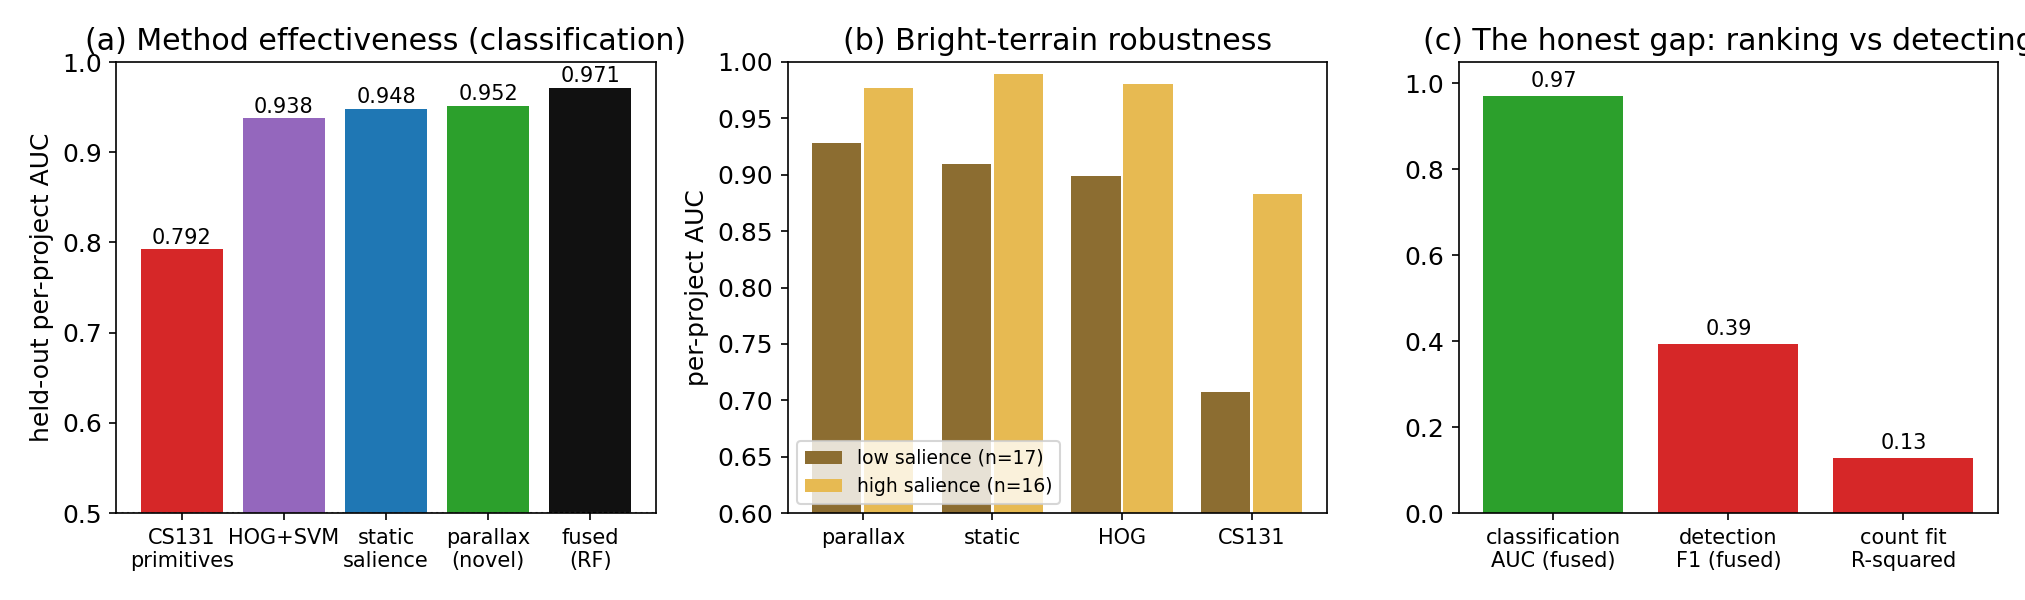
\includegraphics[width=0.98\textwidth]{figs/fig_effectiveness.png}
\caption{(a) Per-method classification effectiveness (held-out per-project AUC): the parallax cue alone beats the appearance baselines and the from-scratch primitives, and the fused model is best. (b) On the bright, low-salience terrain that defeats appearance, parallax is the most robust single family; CS131 primitives collapse to 0.707. (c) The honest gap: the same fused model that ranks at 0.97 AUC commits to detections at only F1 0.39 and counts at $R^2$ 0.13.}
\label{fig:eff}
\end{figure*}

\textbf{Which cues work.} \cref{tab:methods} and \cref{fig:eff}(a) give the headline. The from-scratch CS131 primitives remain weak at 10\,m (per-project AUC 0.792). The two appearance approaches (HOG 0.938, salience 0.948) are strong, and the novel parallax cue is the best single family at 0.952. Fusing parallax with salience reaches 0.971; adding HOG or the CS131 primitives does not help. A leave-one-family-out test on the full random forest (\cref{tab:family}) makes the dependence explicit: removing parallax costs 0.013 AUC, the largest drop, while removing CS131 costs nothing and removing HOG slightly improves the held-out number. The system is, in effect, salience plus motion. Permutation importance on the fused model agrees: the brightness z-score \texttt{stat\_zbright} (mean test-AUC drop 0.011) and the red-blue fringe peak \texttt{plx\_rb\_peak} (0.004) are the two most important features, one from each story.

\begin{table}[t]
\centering
\small
\begin{tabular}{lcc}
\toprule
Family & alone (RF) & drop if removed from full \\
\midrule
Band-parallax & 0.952 & \textbf{0.013} \\
Static salience & 0.953 & 0.002 \\
HOG & 0.937 & $-0.003$ \\
CS131 primitives & 0.804 & 0.000 \\
\bottomrule
\end{tabular}
\caption{Family ablation (held-out per-project AUC). Parallax is the load-bearing family; HOG and CS131 are redundant given salience and parallax.}
\label{tab:family}
\end{table}

\textbf{Inside the CS131 family.} \cref{tab:cs131} isolates each primitive. The family is essentially one feature: the center Sobel gradient energy carries it (solo AUC 0.779; removing it collapses the family from 0.792 to 0.678), Harris adds a little, and the matched template and Hough add nothing. Hough at 0.520 is at chance, the cleanest negative result here: at 10\,m a turbine is a few pixels and its blades are not resolvable line segments, so a line-support primitive has no signal. The whole family lifts per-project AUC by only $+0.012$ on top of salience. This is the central lesson of the static track: classic edge/line/corner primitives, applied directly, degrade to a single ``small bright textured blob'' detector at 10\,m.

\begin{table}[t]
\centering
\small
\begin{tabular}{lcc}
\toprule
CS131 primitive & solo AUC & drop if removed \\
\midrule
center Sobel energy & 0.779 & 0.114 \\
Harris response & 0.681 & 0.010 \\
matched template & 0.635 & 0.003 \\
Hough line support & 0.520 & 0.004 \\
\bottomrule
\end{tabular}
\caption{Per-primitive effect within the CS131 family (held-out per-project AUC). One primitive, the Sobel gradient energy, carries the family; Hough is at chance.}
\label{tab:cs131}
\end{table}

\textbf{Is parallax real motion or re-encoded contrast?} This is the cue's main risk, since a bright turbine produces a band-difference even with still blades, and the fringe peak does correlate with salience ($r{\approx}0.4$--$0.47$). Two train-only controls answer it. Orthogonalizing every parallax feature against the salience features and keeping only the residual still scores per-project AUC 0.763. Holding contrast roughly constant by binning into salience deciles, the best parallax feature separates turbines at within-bin AUC 0.759 (0.82--0.90 in the mid-contrast bins), while the salience cue itself falls to 0.527 (chance) inside the same bins. A label-shuffle control collapses CV AUC to 0.490, confirming no leakage. The parallax family carries genuine motion information beyond contrast.

\textbf{Where each cue wins.} \cref{tab:salience} and \cref{fig:eff}(b) split the test set at median salience. On the bright, textured (low-salience) half, parallax is the most robust family (0.928), the regime that broke the original appearance detector and where the CS131 primitives fall to 0.707. On easy high-salience scenes, static appearance is best and parallax is marginally behind. The two are complementary, which is why the fused model wins.

\begin{table}[t]
\centering
\small
\begin{tabular}{lcccc}
\toprule
Test regime & parallax & static & HOG & CS131 \\
\midrule
Low-salience (17 proj) & \textbf{0.928} & 0.909 & 0.899 & 0.707 \\
High-salience (16 proj) & 0.977 & \textbf{0.990} & 0.980 & 0.883 \\
\bottomrule
\end{tabular}
\caption{Per-project AUC by appearance-salience. Parallax is the most salience-robust family on bright, textured terrain.}
\label{tab:salience}
\end{table}

\textbf{The honest gap, and case studies.} Run as a real detector, the same model scores only F1 0.39 and count $R^2$ 0.13 with slope 0.54 and 58\% mean absolute count error (\cref{fig:eff}(c)): ranking pre-placed candidate points is far easier than committing to detections across a scene with one global threshold. \cref{fig:cases} shows why on re-fetched imagery. The cue is large on the operating fleet at Golden Hills (fringe peak 12.5 vs 2.5 background) and clear even on low-salience terrain at Rockland (3.9 vs 1.4), but it inverts at Roundhouse, WY (turbine 1.08 \emph{below} background 1.71, AUC 0.29) and collapses at Shamrock, TX (48 plainly visible turbines, average fringe 1.58, zero detected). The reason is physical: those fleets were idle at acquisition, so there was no blade motion to read. Conversely, bright terrain causes over-detection: North Hurlburt, OR returns 117 false positives for 24 turbines (recall 0.88, precision 0.15). The cue measures rotation, not presence.

\begin{figure}[t]
\centering
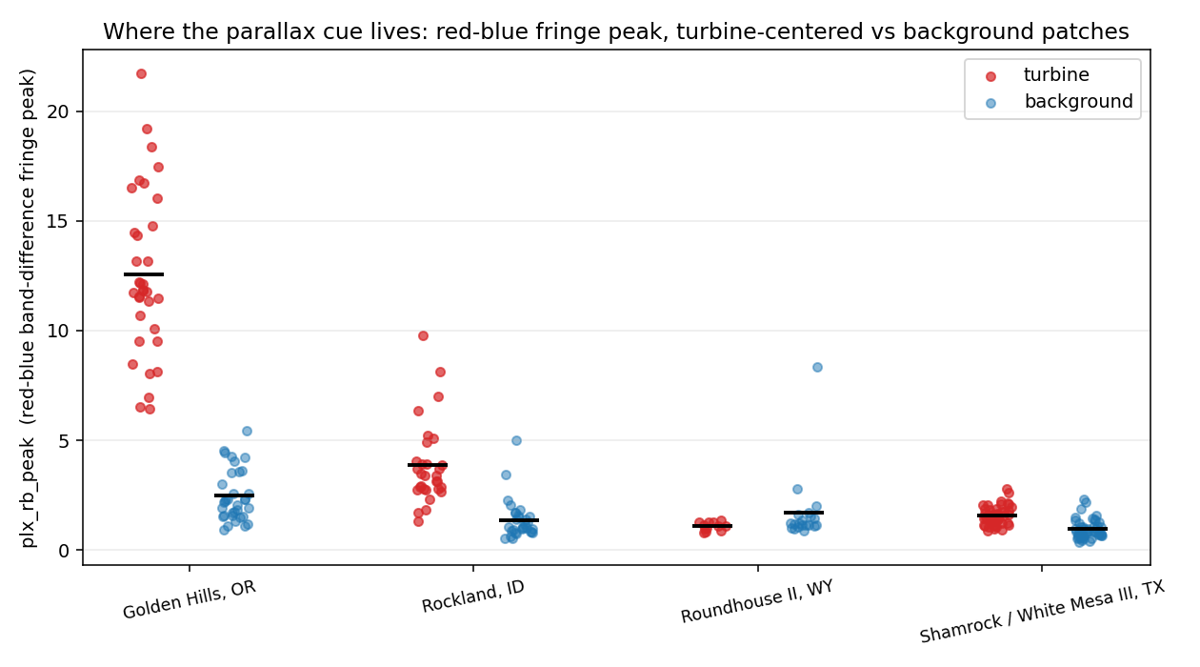
\includegraphics[width=\linewidth]{figs/fig_separation.png}
\caption{Red-blue fringe peak, turbine vs background patches, on four re-fetched projects. The cue separates cleanly when turbines spin (Golden Hills, Rockland) and fails or inverts when they are idle (Roundhouse, Shamrock).}
\label{fig:cases}
\end{figure}

\section{Conclusion}
At 10\,m, the methods that work are static brightness salience and, newly, an interpretable band-parallax cue that reads blade motion; the textbook line/corner/template primitives mostly do not, reducing to a single Sobel-energy ``small bright blob'' feature, and HOG adds nothing over the engineered cues. The parallax cue is the most salience-robust family on exactly the bright terrain where appearance fails, and it is contrast-separable, which prior motion work never showed. We are explicit that this is candidate-point classification: as a real detector the result is weak (F1 0.39), and the cue is structurally blind to idle turbines, capping recall against installed-count ground truth. The most defensible claim is a rigorous, interpretable demonstration that free Sentinel-2 inter-band parallax is an operational-turbine signal worth fusing with appearance. Future work: add hard negatives (buildings, towers) to harden precision, fuse parallax with a static detector and build a true count benchmark against USWTDB/EIA-860, stratify recall by wind speed at acquisition, and use the five-day revisit to recover idle turbines and turn the signal into a nowcast time series.

\section{Individual Contributions}
\textbf{[Author One]} built the data pipeline (panel selection, Sentinel-2 and NAIP fetching, feature matrix) and the leakage-free evaluation harness. \textbf{[Author Two]} implemented the from-scratch CS131 primitives and the HOG/salience baselines, and ran the classifier sweep and ablations. \textbf{[Author Three]} designed and implemented the band-parallax features, the contrast-separability controls, the detection-mode benchmark, and the case studies. All authors contributed to the experimental design, analysis, and writing. \emph{(Replace bracketed names and adjust the specific code/experiments each member owned.)}

{\small
\bibliographystyle{plain}
\begin{thebibliography}{99}
\bibitem{uswtdb} USGS, AWEA, LBNL. The U.S. Wind Turbine Database (USWTDB). \url{https://eerscmap.usgs.gov/uswtdb/}, 2024.
\bibitem{grw} C. Robinson \etal. Global Renewables Watch: A Temporal Dataset of Solar and Wind Energy Derived from Satellite Imagery. arXiv:2503.14860, 2025.
\bibitem{satlas} F. Bastani \etal. SatlasPretrain: A Large-Scale Dataset for Remote Sensing Image Understanding. ICCV, 2023.
\bibitem{dunnett} S. Dunnett \etal. Harmonised global datasets of wind and solar farm locations and power. Scientific Data, 7:130, 2020.
\bibitem{mandroux_ipol} N. Mandroux, T. Dagobert, S. Drouyer, R. Grompone von Gioi. Single Date Wind Turbine Detection on Sentinel-2 Optical Images. Image Processing On Line, 12:198--217, 2022.
\bibitem{mandroux_isprs} N. Mandroux, S. Drouyer, R. Grompone von Gioi. Multi-Date Wind Turbine Detection on Optical Satellite Images. ISPRS Annals, V-2-2022:383--390, 2022.
\bibitem{he2025} J. He \etal. Mapping land- and offshore-based wind turbines in China with Sentinel-2 satellite data. Renewable and Sustainable Energy Reviews, 2025.
\bibitem{nahrstedt} F. Nahrstedt, P. G\"artner, J. Wittmann. Detection of wind turbine motion between satellite bands with convolutional neural networks. EnviroInfo, 2023.
\bibitem{heiselberg} H. Heiselberg. Aircraft and Ship Velocity Determination in Sentinel-2 Multispectral Images. Sensors, 19(13):2873, 2019.
\bibitem{liu} W. Liu \etal. Space eye on flying aircraft: From Sentinel-2 MSI parallax to hybrid computing. Remote Sensing of Environment, 246:111867, 2020.
\bibitem{wtyolo} L. Zhai, X. Chen \etal. Identifying wind turbines from multiresolution and multibackground remote sensing imagery. Int. J. Applied Earth Observation and Geoinformation, 122:103613, 2023.
\bibitem{deepowt} T. Hoeser, S. Feuerstein, C. Kuenzer. DeepOWT: a global offshore wind turbine data set derived with deep learning from Sentinel-1 data. Earth System Science Data, 14:4251--4270, 2022.
\bibitem{dalal} N. Dalal, B. Triggs. Histograms of Oriented Gradients for Human Detection. CVPR, 2005.
\bibitem{harris} C. Harris, M. Stephens. A Combined Corner and Edge Detector. Alvey Vision Conference, 1988.
\end{thebibliography}
}

\appendix
\section{Full band-parallax feature list}
\label{app:features}
All 19 features are computed after per-band high-pass (subtract a $\sigma{=}3$ Gaussian) and z-normalization. \textbf{Band-difference fringe maps} for red-blue (rb), green-blue (gb), and red-green (rg), each summarized over the central window by: peak $|\cdot|$, peak-to-peak, mean energy, and dipole separation (distance between the strongest positive and negative lobes), giving 12 features. \textbf{Chromatic dispersion} across the three visible bands: central mean and peak (2). \textbf{Cross-correlation} of blue to red: integer offset magnitude, peak correlation, and decorrelation $1{-}\text{peak}$ (3). \textbf{Time-ordering consistency}: correlation between the rb and gb central fringe maps (1), since red lags blue more than green does. \textbf{Energy ratio} rb/gb (1). The whole-patch cross-correlation offset proved nearly useless (about 0 for both classes, since the static ground dominates the global alignment); the signal lives in the localized fringe energy, and permutation importance confirms this feature carries almost no weight.

\section{Classifier sweep (train, GroupKFold CV AUC)}
\label{app:sweep}
\begin{table}[h]
\centering
\small
\begin{tabular}{lcc}
\toprule
Feature family & logistic reg. & best of 5 models \\
\midrule
CS131 primitives only & 0.782 & 0.782 \\
Static (stat+cv131) & 0.943 & 0.960 (XGB) \\
HOG & 0.934 & 0.934 \\
Parallax only & 0.952 & 0.960 (RF) \\
Parallax + static & 0.973 & 0.979 (XGB) \\
All families & 0.974 & 0.980 (XGB) \\
\bottomrule
\end{tabular}
\caption{Pooled GroupKFold(5) CV AUC on train only. Five classifiers (logistic regression, RBF-SVM, random forest, XGBoost, MLP) were CV-tuned; the headline model (RF on parallax+static) was selected by per-project CV AUC (0.967) and frozen before the single test pass.}
\end{table}

\section{Case-study detail}
\label{app:cases}
\Cref{fig:grid} shows one representative (strongest-fringe) turbine per case project: a strong fringe at Golden Hills, a clear one at Rockland on low-salience terrain, and a collapse at Roundhouse and Shamrock where the fleets were idle and plainly visible in true color but produced no motion fringe. Detection-mode per-project F1 ranged from 0.00 (Shamrock, Roundhouse, Chevelon Butte) to 0.69 (Stetson, ME).

\begin{figure}[h]
\centering
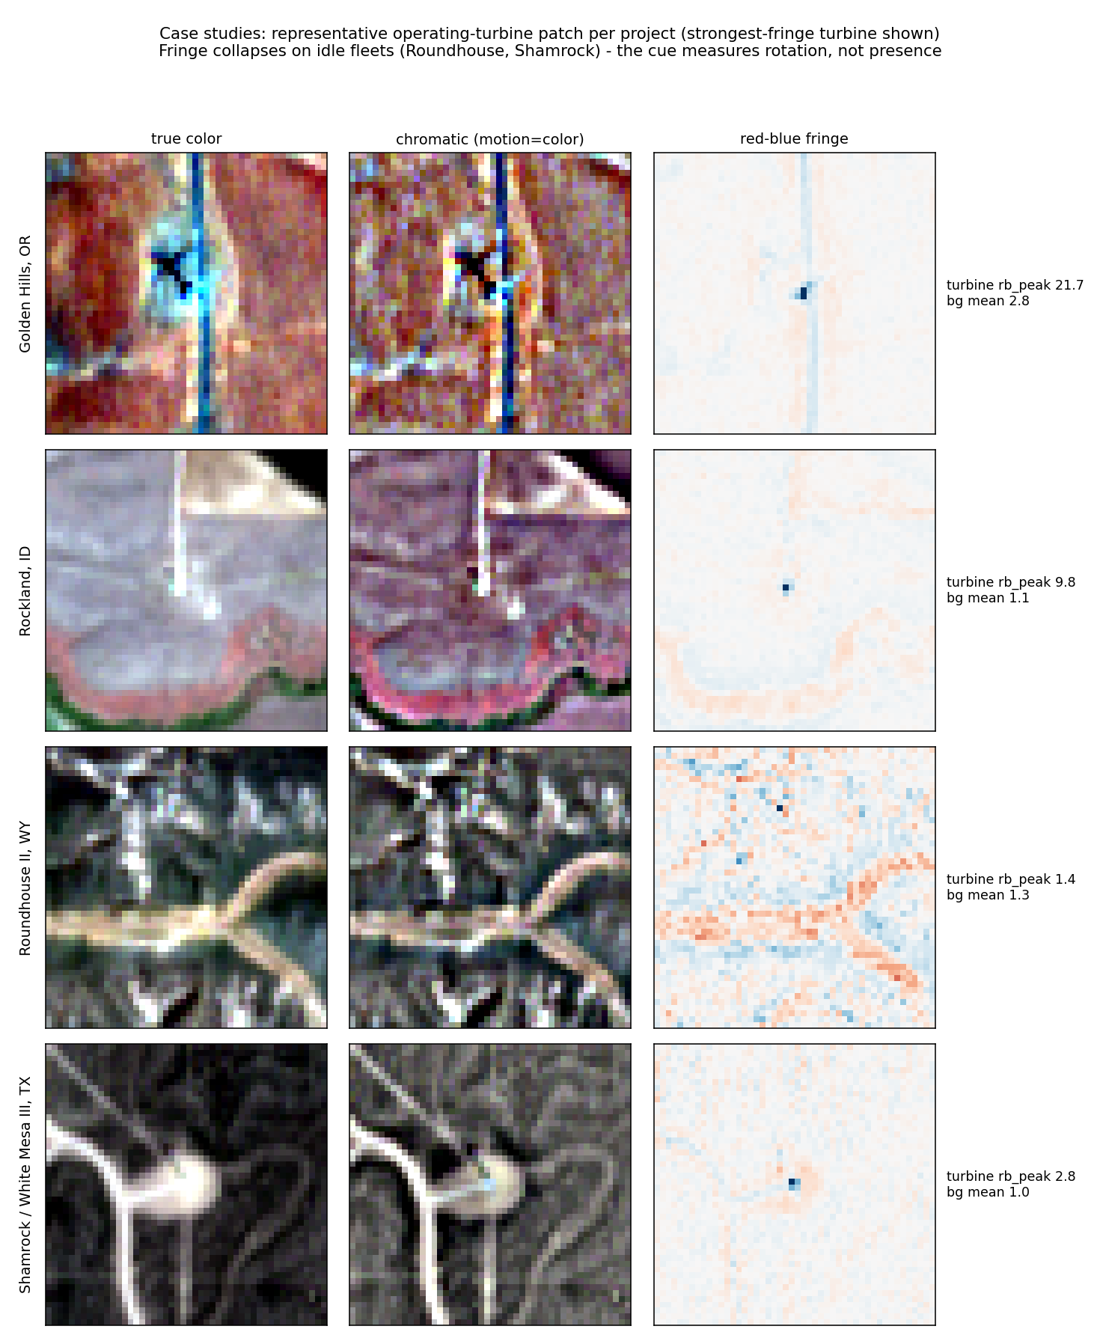
\includegraphics[width=0.92\linewidth]{figs/fig_grid.png}
\caption{Representative turbine per case project: true color, chromatic high-pass composite, and red-blue fringe map. The fringe collapses on idle fleets, illustrating the rotation-not-presence limit.}
\label{fig:grid}
\end{figure}

\section{Reproducibility}
\label{app:repro}
All numbers were regenerated from a cached feature matrix and a frozen model; the headline detectors reproduced to three decimals. Ablation traces (single-feature AUC, CS131 primitive effect, family ablation, permutation importance, salience stratification) are saved as JSON/CSV, and the four case-study chips were re-fetched live from Sentinel-2 via AWS Earth Search, with the parallax pipeline recomputed from raw bands (matching the matrix to two decimals).

\end{document}
